\chapter{Hashing and Hash Tables}\label{ch08:hashing-and-hash-tables}

\section{Introduction}

> \textbf{Complete compilable implementations of the data structures in this chapter are in \texttt{code/}.}

\section{The Dictionary ADT}

A \textbf{dictionary} (also called map or associative array) stores key-value pairs and supports:

\begin{itemize}
\item \textbf{insert(key, value)} — add a new key-value pair
\item \textbf{find(key)} — return the value associated with key
\item \textbf{erase(key)} — remove the key-value pair
\end{itemize}

Hash tables implement dictionaries with average O(1) time per operation — a dramatic improvement over the O(log n) of balanced trees.

\section{Hash Tables: Basic Idea}

A \textbf{hash table} uses a \textbf{hash function} h(k) to map each key k to an index in an array of size m. The pair (k, v) is stored at position h(k) in the table.

\begin{figure}[ht]
\centering
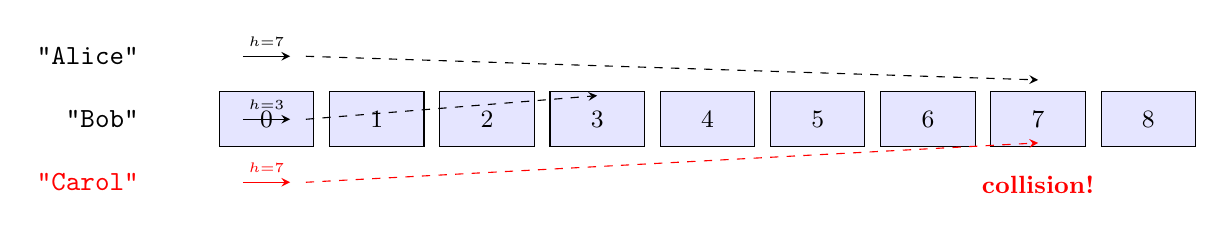
\begin{tikzpicture}
\tikzstyle{entry}=[draw,rectangle,minimum width=1.2cm,minimum height=0.7cm,inner sep=2pt]
\tikzstyle{nullbox}=[draw,rectangle,minimum width=0.5cm,minimum height=0.7cm,inner sep=2pt]

% Hash table array
\foreach \i/\lbl in {0/{\small 0},1/{\small 1},2/{\small 2},3/{\small 3},4/{\small 4},
                      5/{\small 5},6/{\small 6},7/{\small 7},8/{\small 8}} {
  \node[entry,fill=blue!10] (t\i) at (\i*1.4,0) {\lbl};
}

% Alice -> 7
\node[anchor=east] at (-1.5,0.8) {\texttt{"Alice"}};
\draw[->,>=stealth] (-0.3,0.8) -- (0.3,0.8) node[midway,above] {\tiny $h$=7};
\draw[->,>=stealth,dashed] (0.5,0.8) -- (7*1.4,0.5);

% Bob -> 3
\node[anchor=east] at (-1.5,0) {\texttt{"Bob"}};
\draw[->,>=stealth] (-0.3,0) -- (0.3,0) node[midway,above] {\tiny $h$=3};
\draw[->,>=stealth,dashed] (0.5,0) -- (3*1.4,0.3);

% Carol -> 7 (collision)
\node[anchor=east,text=red] at (-1.5,-0.8) {\texttt{"Carol"}};
\draw[->,>=stealth,red] (-0.3,-0.8) -- (0.3,-0.8) node[midway,above] {\tiny $h$=7};
\draw[->,>=stealth,dashed,red] (0.5,-0.8) -- (7*1.4,-0.3);
\node[red,below] at (7*1.4,-0.6) {\small\bfseries collision!};
\end{tikzpicture}
\end{figure}

When two keys hash to the same index, we have a \textbf{collision}. Collision resolution is the central challenge of hash table design.

\section{Hash Functions}

\subsection{Properties of a Good Hash Function}

\begin{enumerate}
\item \textbf{Deterministic} — same key always produces the same hash
\item \textbf{Uniform} — keys are distributed evenly across the table
\item \textbf{Fast} — O(1) to compute
\item \textbf{Non-invertible} — hard to reconstruct the key from the hash (not a security requirement for general hashing, but good practice)
\end{enumerate}

\subsection{Integer Keys}

For integer keys, the simplest approach: \textbf{h(k) = k mod m}.

m should be prime to reduce patterns. For example, m = 13:
\begin{lstlisting}[language=Java]
h(10) = 10 mod 13 = 10
h(26) = 26 mod 13 = 0
h(39) = 39 mod 13 = 0  // collision with 26!
\end{lstlisting}

\subsection{String Keys}

\begin{lstlisting}[language=C++]
// djb2 hash -- simple but effective
size_t hash_string(std::string_view s) {
    size_t h = 5381;
    for (char c : s) {
        h = h * 33 + static_cast<size_t>(c);
    }
    return h;
}
\end{lstlisting}

\subsection{Rob Dixon's "sdbm" hash}

\begin{lstlisting}[language=C++]
size_t hash_sdbm(std::string_view s) {
    size_t h = 0;
    for (char c : s) {
        h = c + (h << 6) + (h << 16) - h;
    }
    return h;
}
\end{lstlisting}

\subsection{std::hash}

C++ provides \texttt{std::hash<T>} for common types:

\begin{lstlisting}[language=C++]
std::hash<int> int_hash;
size_t h = int_hash(42);

std::hash<std::string> str_hash;
size_t h2 = str_hash("hello");

// Custom hash for user types:
struct point {
    int x, y;
    bool operator==(const point& other) const {
        return x == other.x && y == other.y;
    }
};

template <>
struct std::hash<point> {
    size_t operator()(const point& p) const noexcept {
        size_t h1 = std::hash<int>{}(p.x);
        size_t h2 = std::hash<int>{}(p.y);
        return h1 ^ (h2 << 1);
    }
};
\end{lstlisting}

\section{Separate Chaining}

Each table slot holds a linked list (or any container) of all key-value pairs that hash to that position.

\begin{figure}[ht]
\centering
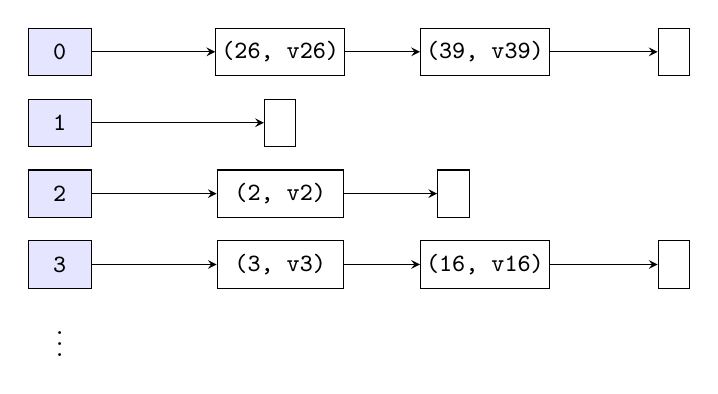
\begin{tikzpicture}
\tikzstyle{bucket}=[draw,rectangle,minimum width=0.8cm,minimum height=0.6cm,inner sep=2pt]
\tikzstyle{chainnode}=[draw,rectangle,minimum width=1.6cm,minimum height=0.6cm,inner sep=2pt]
\tikzstyle{nullbox}=[draw,rectangle,minimum width=0.4cm,minimum height=0.6cm,inner sep=2pt]

% Buckets
\node[bucket,fill=blue!10] (b0) at (0,0)      {\small\tt 0};
\node[bucket,fill=blue!10] (b1) at (0,-0.9)   {\small\tt 1};
\node[bucket,fill=blue!10] (b2) at (0,-1.8)   {\small\tt 2};
\node[bucket,fill=blue!10] (b3) at (0,-2.7)   {\small\tt 3};
\node at (0,-3.6) {$\vdots$};

% Chain entries
\node[chainnode] (c0) at (2.8,0)    {\small\tt(26,\ v26)};
\draw[->,>=stealth] (b0.east) -- (c0.west);
\node[chainnode] (c0b) at (5.4,0)   {\small\tt(39,\ v39)};
\draw[->,>=stealth] (c0.east) -- (c0b.west);
\node[nullbox] (c0c) at (7.8,0)     {$\varnothing$};
\draw[->,>=stealth] (c0b.east) -- (c0c.west);

\node[nullbox] (c1) at (2.8,-0.9)  {$\varnothing$};
\draw[->,>=stealth] (b1.east) -- (c1.west);

\node[chainnode] (c2) at (2.8,-1.8) {\small\tt(2,\ v2)};
\draw[->,>=stealth] (b2.east) -- (c2.west);
\node[nullbox] (c2b) at (5.0,-1.8) {$\varnothing$};
\draw[->,>=stealth] (c2.east) -- (c2b.west);

\node[chainnode] (c3) at (2.8,-2.7) {\small\tt(3,\ v3)};
\draw[->,>=stealth] (b3.east) -- (c3.west);
\node[chainnode] (c3b) at (5.4,-2.7) {\small\tt(16,\ v16)};
\draw[->,>=stealth] (c3.east) -- (c3b.west);
\node[nullbox] (c3c) at (7.8,-2.7) {$\varnothing$};
\draw[->,>=stealth] (c3b.east) -- (c3c.west);
\end{tikzpicture}
\end{figure}

\begin{lstlisting}[language=C++]
template <typename K, typename V, typename Hash = std::hash<K>>
class hash_table_chaining {
public:
    explicit hash_table_chaining(size_t initial_buckets = 16)
        : buckets_(initial_buckets), table_(initial_buckets) {}

    void insert(const K& key, const V& value) {
        auto& chain = table_[bucket(key)];
        for (auto& [k, v] : chain) {
            if (k == key) {
                v = value;  // update existing
                return;
            }
        }
        chain.push_back({key, value});
        ++size_;
        check_load();
    }

    std::optional<V> find(const K& key) const {
        const auto& chain = table_[bucket(key)];
        for (const auto& [k, v] : chain) {
            if (k == key) return v;
        }
        return std::nullopt;
    }

    void erase(const K& key) {
        auto& chain = table_[bucket(key)];
        auto it = std::find_if(chain.begin(), chain.end(),
            [&](const auto& p) { return p.first == key; });
        if (it != chain.end()) {
            chain.erase(it);
            --size_;
        }
    }

    size_t size() const noexcept { return size_; }
    bool empty() const noexcept { return size_ == 0; }

private:
    size_t bucket(const K& key) const {
        return Hash{}(key) % buckets_;
    }

    void check_load() {
        // Rehash when load factor exceeds 1.0
        if (size_ > buckets_) {
            buckets_ *= 2;
            std::vector<std::list<std::pair<K, V>>> new_table(buckets_);
            for (const auto& chain : table_) {
                for (const auto& pair : chain) {
                    size_t b = Hash{}(pair.first) % buckets_;
                    new_table[b].push_back(pair);
                }
            }
            table_ = std::move(new_table);
        }
    }

    size_t buckets_;
    size_t size_ = 0;
    std::vector<std::list<std::pair<K, V>>> table_;
};
\end{lstlisting}

\textbf{Load factor:} $\alpha $ = n/m (number of elements / number of buckets). With separate chaining, $\alpha $ can exceed 1. Average chain length = $\alpha $.

\section{Open Addressing}

All elements are stored in the table array itself. On collision, we probe for the next empty slot.

\subsection{Linear Probing}

If slot h(k) is occupied, try h(k) + 1, h(k) + 2, ..., wrapping around.

\begin{figure}[ht]
\centering
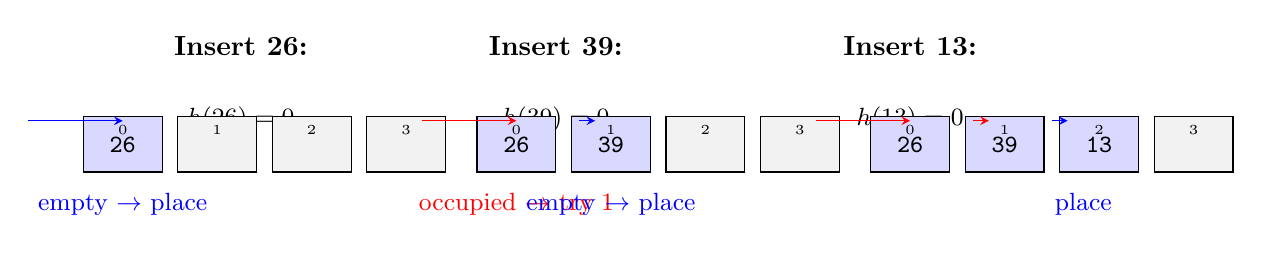
\begin{tikzpicture}
\tikzstyle{slot}=[draw,rectangle,minimum width=1cm,minimum height=0.7cm,inner sep=2pt]

% Step 1: insert 26
\node[above] at (1.5,0.5) {\textbf{Insert 26:}};
\node[below] at (1.5,0.1) {\small$h(26)=0$};
\foreach \i/\lbl/\clr in {0/26/blue!15,1//gray!10,2//gray!10,3//gray!10} {
  \node[slot,fill=\clr] (s\i) at (\i*1.2,-0.5) {\small\tt\lbl};
  \node[above] at (\i*1.2,-0.5) {\tiny\i};
}
\draw[->,>=stealth,blue] (-1.2,-0.2) -- (0,-0.2);
\node[below,blue] at (0,-1.0) {\small empty $\rightarrow$ place};

% Step 2: insert 39
\node[above] at (5.5,0.5) {\textbf{Insert 39:}};
\node[below] at (5.5,0.1) {\small$h(39)=0$};
\foreach \i/\lbl/\clr in {0/26/blue!15,1/39/blue!15,2//gray!10,3//gray!10} {
  \node[slot,fill=\clr] (t\i) at (5+\i*1.2,-0.5) {\small\tt\lbl};
  \node[above] at (5+\i*1.2,-0.5) {\tiny\i};
}
\draw[->,>=stealth,red] (3.8,-0.2) -- (5,-0.2);
\node[below,red] at (5,-1.0) {\small occupied $\rightarrow$ try 1};
\draw[->,>=stealth,blue] (5.8,-0.2) -- (6,-0.2);
\node[below,blue] at (6.2,-1.0) {\small empty $\rightarrow$ place};

% Step 3: insert 13
\node[above] at (10,0.5) {\textbf{Insert 13:}};
\node[below] at (10,0.1) {\small$h(13)=0$};
\foreach \i/\lbl/\clr in {0/26/blue!15,1/39/blue!15,2/13/blue!15,3//gray!10} {
  \node[slot,fill=\clr] (u\i) at (10+\i*1.2,-0.5) {\small\tt\lbl};
  \node[above] at (10+\i*1.2,-0.5) {\tiny\i};
}
\draw[->,>=stealth,red] (8.8,-0.2) -- (10,-0.2);
\draw[->,>=stealth,red] (10.8,-0.2) -- (11,-0.2);
\draw[->,>=stealth,blue] (11.8,-0.2) -- (12,-0.2);
\node[below,blue] at (12.2,-1.0) {\small place};
\end{tikzpicture}
\end{figure}

\textbf{Problem: primary clustering.} A block of consecutive occupied slots grows, attracting more collisions.

\subsection{Quadratic Probing}

Try positions: h(k), h(k) + 1$^{2}$, h(k) + 2$^{2}$, h(k) + 3$^{2}$, ...

\begin{lstlisting}[language=Java]
Probe sequence: p(i) = (h(k) + i$^{2}$) mod m
\end{lstlisting}

Reduces clustering but may miss slots even when the table is not full.

\subsection{Double Hashing}

Use a second hash function for the probe step:

\begin{lstlisting}[language=Java]
Probe sequence: p(i) = (h(k) + i$\cdot$h$_{2}$(k)) mod m
\end{lstlisting}

This gives the best distribution of the three open addressing methods.

\begin{lstlisting}[language=C++]
template <typename K, typename V, typename Hash = std::hash<K>>
class hash_table_open {
public:
    explicit hash_table_open(size_t initial_capacity = 16)
        : capacity_(initial_capacity), size_(0),
          states_(initial_capacity, State::empty),
          keys_(initial_capacity), values_(initial_capacity) {}

    bool insert(const K& key, const V& value) {
        if (size_ >= capacity_ * 0.7) rehash();
        size_t i = 0;
        size_t pos;
        do {
            pos = probe(key, i);
            if (states_[pos] == State::empty || states_[pos] == State::deleted) {
                keys_[pos] = key;
                values_[pos] = value;
                states_[pos] = State::occupied;
                ++size_;
                return true;
            }
            if (states_[pos] == State::occupied && keys_[pos] == key) {
                values_[pos] = value;  // update
                return false;
            }
            ++i;
        } while (i < capacity_);
        rehash();
        return insert(key, value);
    }

    std::optional<V> find(const K& key) const {
        size_t i = 0;
        size_t pos;
        do {
            pos = probe(key, i);
            if (states_[pos] == State::empty) return std::nullopt;
            if (states_[pos] == State::occupied && keys_[pos] == key) {
                return values_[pos];
            }
            ++i;
        } while (i < capacity_);
        return std::nullopt;
    }

    void erase(const K& key) {
        size_t i = 0;
        size_t pos;
        do {
            pos = probe(key, i);
            if (states_[pos] == State::empty) return;
            if (states_[pos] == State::occupied && keys_[pos] == key) {
                states_[pos] = State::deleted;
                --size_;
                return;
            }
            ++i;
        } while (i < capacity_);
    }

private:
    enum class State { empty, occupied, deleted };

    size_t probe(const K& key, size_t i) const {
        size_t h1 = Hash{}(key) % capacity_;
        size_t h2 = 1 + (Hash{}(key) % (capacity_ - 1));  // second hash
        return (h1 + i * h2) % capacity_;
    }

    void rehash() {
        size_t old_cap = capacity_;
        capacity_ *= 2;
        std::vector<State> old_states = std::move(states_);
        std::vector<K> old_keys = std::move(keys_);
        std::vector<V> old_values = std::move(values_);

        states_ = std::vector<State>(capacity_, State::empty);
        keys_.resize(capacity_);
        values_.resize(capacity_);
        size_ = 0;

        for (size_t i = 0; i < old_cap; ++i) {
            if (old_states[i] == State::occupied) {
                insert(old_keys[i], old_values[i]);
            }
        }
    }

    size_t capacity_, size_;
    std::vector<State> states_;
    std::vector<K> keys_;
    std::vector<V> values_;
};
\end{lstlisting}

\section{Skip Lists}

A \textbf{skip list} is a probabilistic data structure that maintains an ordered set with O(log n) expected time for search, insert, and erase. It consists of multiple linked levels, where each higher level acts as an "express lane" over the level below.

\subsection{Structure}

A skip list is a hierarchy of sorted linked lists:

\begin{lstlisting}[language=Java]
level 3:  1 --------------------------- ->  9
level 2:  1 ----------- ->  5 ----------- ->  9
level 1:  1 --- ->  3 --- ->  5 --- ->  7 --- ->  9
level 0:  1  ->  2  ->  3  ->  4  ->  5  ->  6  ->  7  ->  8  ->  9  ->  {empty}
\end{lstlisting}

Each element appears in level 0. It appears in higher levels with probability 1/2 per level (i.e., level 1: 1/2, level 2: 1/4, level 3: 1/8, etc.). The maximum level is typically capped at $\lceil $log$_{2}$ n$\rceil $.

\subsection{Node Structure}

\begin{lstlisting}[language=C++]
template <typename K, typename V>
struct skip_node {
    K key;
    V value;
    std::vector<skip_node*> next;  // next[i] = successor at level i

    skip_node(const K& k, const V& v, int level)
        : key(k), value(v), next(level + 1, nullptr) {}
};
\end{lstlisting}

\subsection{Search}

Search proceeds from the topmost level, moving forward as far as possible at each level before descending:

\begin{lstlisting}[language=C++]
template <typename K, typename V>
V* skip_list<K, V>::find(const K& key) {
    auto* cur = head_;
    for (int i = level_; i >= 0; --i) {
        while (cur->next[i] && cur->next[i]->key < key)
            cur = cur->next[i];
    }
    cur = cur->next[0];
    if (cur && cur->key == key) return &cur->value;
    return nullptr;
}
\end{lstlisting}

\subsection{Insertion}

To insert, we search through all levels and record the nodes where we need to insert at each level. We then choose a random level for the new node and link it in:

\begin{lstlisting}[language=C++]
template <typename K, typename V>
void skip_list<K, V>::insert(const K& key, const V& value) {
    std::vector<skip_node<K, V>*> update(level_ + 1, nullptr);
    auto* cur = head_;

    for (int i = level_; i >= 0; --i) {
        while (cur->next[i] && cur->next[i]->key < key)
            cur = cur->next[i];
        update[i] = cur;
    }

    cur = cur->next[0];
    if (cur && cur->key == key) {
        cur->value = value;  // key already exists
        return;
    }

    int new_level = random_level();
    if (new_level > level_) {
        head_->next.resize(new_level + 1, nullptr);
        update.resize(new_level + 1, head_);
        level_ = new_level;
    }

    auto* node = new skip_node<K, V>(key, value, new_level);
    for (int i = 0; i <= new_level; ++i) {
        node->next[i] = update[i]->next[i];
        update[i]->next[i] = node;
    }
}
\end{lstlisting}

\subsection{Choosing the Level}

\begin{lstlisting}[language=C++]
int random_level() {
    int level = 0;
    while (rand() < RAND_MAX / 2 && level < MAX_LEVEL)
        ++level;
    return level;
}
\end{lstlisting}

This produces level 0 with probability 1/2, level 1 with probability 1/4, level 2 with probability 1/8, etc.

\subsection{Complexity}

\begin{center}
\begin{tabular}{ccc}
\toprule
Operation & Expected & Worst Case \\
Search & O(log n) & O(n) \\
Insert & O(log n) & O(n) \\
Erase & O(log n) & O(n) \\
Space & O(n) & O(n log n) \\

\bottomrule
\end{tabular}
\end{center}
The worst case occurs when all elements get the same level (e.g., all level 0). The probability of this is vanishingly small: (1/2)$^{n}$ for n elements all at level 0.

\subsection{Skip Lists vs. Hash Tables vs. Balanced Trees}

\begin{center}
\begin{tabular}{cccc}
\toprule
Criteria & Hash Table & Skip List & Balanced Tree \\
Average search & O(1) & O(log n) & O(log n) \\
Ordered iteration & No & O(n log n) & O(n) in-order \\
Range queries & No & O(log n + k) & O(log n + k) \\
Implementation & Medium & Medium & Complex \\
Memory & O(n + m) & O(n) expected & O(n) \\

\bottomrule
\end{tabular}
\end{center}
Skip lists occupy a useful middle ground: they support ordered operations like balanced trees but are much simpler to implement. They are not a replacement for hash tables (which are faster for unordered lookups), but they are competitive with balanced trees for ordered maps.

\subsection{STL Connection}

The C++ standard library does not include a skip list implementation. However, the \texttt{leveldb} and \texttt{rocksdb} databases use skip lists as their default in-memory table implementation, and Redis uses skip lists for sorted sets.

\section{Modern Hash Table Designs}

\subsection{Robin Hood Hashing}

When probing, if the current occupant is "richer" (closer to its ideal position) than the incoming element, swap them. This equalizes probe distances.

\begin{lstlisting}[language=Java]
Insert 39: h(39)=0  ->  occupied by 26 (probe distance 0)
           Compare: 39 has distance 0, 26 has distance 0  ->  keep going
           Try 1  ->  empty  ->  insert 39 (distance 1)

Insert 13: h(13)=0  ->  26 (dist 0)  ->  compare equal  ->  keep going
           1  ->  39 (dist 1)  ->  compare equal  ->  keep going
           2  ->  empty  ->  insert (dist 2)

Insert 1:  h(1)=1  ->  39 (dist 1)  ->  1 has dist 0 < 39's dist 1  ->  keep going
           2  ->  13 (dist 2)  ->  1 has dist 1 < 13's dist 2  ->  keep going
           3  ->  empty  ->  insert (dist 3)
\end{lstlisting}

\subsection{Cuckoo Hashing}

Use two hash tables with two different hash functions. On collision, evict the existing element and insert it into the other table. If this cycles, rehash.

\subsection{Swiss Table (Google's Abseil flat\_hash\_map)}

Uses SIMD (SSE2/ARM NEON) to probe 16 slots simultaneously. Each slot has a 1-byte metadata field (7 bits of hash + 1 bit for occupancy). The lookup checks all 16 metadata bytes in one CPU instruction.

\begin{lstlisting}[language=C++]
// Abseil flat_hash_map -- the fastest general-purpose hash table
#include <absl/container/flat_hash_map.h>

absl::flat_hash_map<std::string, int> map;
map["hello"] = 1;
map["world"] = 2;
\end{lstlisting}

\section{Distributed Hash Table (DHT)}

\subsection{Introduction}

A \textbf{distributed hash table} (DHT) distributes key-value pairs across many nodes in a peer-to-peer (P2P) network. Each node owns a contiguous range of keys and is responsible for storing all key-value pairs in that range. Unlike a centralized hash table where one server handles all lookups, a DHT spreads the storage and query load across $n$ participating nodes.

The key idea is \textbf{consistent hashing}: both keys and node identifiers occupy the same circular address space (typically $[0, 2^m - 1]$). A key is assigned to the first node whose identifier is equal to or greater than the key's hash. This means adding or removing a node only affects keys in its immediate range, not the entire table.

\subsection{Chord Ring Structure}

The Chord protocol arranges nodes in a logical ring. Each node maintains a \textbf{finger table} of $m$ entries that allow it to skip roughly half the ring at each hop, giving $O(\log n)$ lookup.

\begin{verbatim}
    Chord Ring with 8 nodes (m = 3, identifiers 0..7)
    Nodes: 0, 1, 3, 4, 6, 7

              0
           /     \
         7         1
         |    *    |        * = node exists
         6         2        . = empty position
           \     /          Keys 0,1,3,4,6,7 are owned
              5              by the next node clockwise.

    Key ownership (consistent hashing):
      Key 0 -> Node 0      Key 4 -> Node 4
      Key 1 -> Node 1      Key 5 -> Node 6
      Key 2 -> Node 3      Key 6 -> Node 6
      Key 3 -> Node 3      Key 7 -> Node 7

    Node 3 finger table:
      Entry 0: successor of (3+1) mod 8  = 4  ->  Node 4
      Entry 1: successor of (3+2) mod 8  = 5  ->  Node 6
      Entry 2: successor of (3+4) mod 8  = 7  ->  Node 7

    Lookup for key 5 starting at Node 3:
      Step 1: 5 > 3, closest finger <= 5 is Node 4 (entry 0)
      Step 2: at Node 4, 5 in (4, 7] -> forward to Node 6
      Step 3: Node 6 owns key 5.  Done in 2 hops.
\end{verbatim}

\subsection{Simplified C++ Implementation}

The following code simulates a single DHT node with a finger table and basic key-value storage. In a real system, each node would communicate with others over the network.

\begin{lstlisting}[language=C++]
#include <vector>
#include <map>
#include <string>
#include <functional>
#include <cmath>
#include <algorithm>

class DHTNode {
    int id;                        // this node's identifier
    int m;                         // number of bits in id space
    std::vector<int> fingerTable;  // successor for each finger
    std::map<int, std::string> store;  // local key-value storage

    // Compute the start of finger i: (id + 2^i) mod 2^m
    int fingerStart(int i) const {
        return (id + (1 << i)) % (1 << m);
    }

public:
    DHTNode(int nodeId, int bits)
        : id(nodeId), m(bits), fingerTable(bits) {
        for (int i = 0; i < m; i++)
            fingerTable[i] = id;  // placeholder
    }

    int getId() const { return id; }

    // Find the successor node responsible for a given key
    // Uses finger table to skip ahead -- O(log n) hops
    DHTNode* find_successor(DHTNode* allNodes[], int n,
                            int key) {
        // Check if key falls in (this, successor]
        int succ = fingerTable[0];
        if (key > id && key <= succ)
            return this;

        // Find closest preceding node using finger table
        DHTNode* next = nullptr;
        for (int i = m - 1; i >= 0; i--) {
            if (fingerTable[i] > id &&
                fingerTable[i] < key) {
                // In a real system, we would contact
                // the node with this id over the network
                for (int j = 0; j < n; j++) {
                    if (allNodes[j]->id == fingerTable[i]) {
                        next = allNodes[j];
                        break;
                    }
                }
                break;
            }
        }
        if (!next) next = this;  // wrap around

        // Recurse: delegate lookup to the next node
        return next->find_successor(allNodes, n, key);
    }

    // Insert a key-value pair
    void put(int key, const std::string& value) {
        store[key] = value;
    }

    // Retrieve a value by key
    std::string get(int key) const {
        auto it = store.find(key);
        if (it != store.end()) return it->second;
        return "";
    }

    // Build finger table given the full set of nodes
    void buildFingers(DHTNode* allNodes[], int n) {
        for (int i = 0; i < m; i++) {
            int start = fingerStart(i);
            int best = allNodes[0]->id;
            for (int j = 0; j < n; j++) {
                int nid = allNodes[j]->id;
                if (nid >= start) {
                    best = nid;
                    break;
                }
            }
            fingerTable[i] = best;
        }
    }
};
\end{lstlisting}

\subsection{Complexity Analysis}

\begin{center}
\begin{tabular}{lcc}
\toprule
Operation & Time & Notes \\
\midrule
Lookup (find\_successor) & $O(\log n)$ & finger table skips \\
Insert (with stabilization) & $O(\log^2 n)$ & $O(\log n)$ hops $\times$ $O(\log n)$ fixup \\
Node join & $O(\log^2 n)$ & stabilize fingers and predecessors \\
Space per node & $O(\log n)$ & one finger table entry per bit \\
\bottomrule
\end{tabular}
\end{center}

The $O(\log n)$ lookup bound holds because the finger table doubles the distance covered at each step, similar to binary search. Insert stabilization is $O(\log^2 n)$ because a new node must fix $O(\log n)$ fingers, and each fix may require $O(\log n)$ hops to reach the correct node.

\subsection{Applications}

\begin{itemize}
    \item \textbf{BitTorrent} -- Uses a DHT (Kademlia-based) so peers can find each other without a central tracker. Each torrent forms its own DHT overlay.
    \item \textbf{IPFS} -- Uses a Kademlia DHT to locate content by its hash across a global P2P network.
    \item \textbf{Amazon DynamoDB} -- Uses consistent hashing to partition data across storage nodes, inspired by the DHT designs from the early 2000s.
    \item \textbf{Apache Cassandra} -- Uses consistent hashing (via a token ring) to distribute data across a cluster of nodes, handling replication and fault tolerance.
\end{itemize}

\subsection{DHT vs.\ Centralized Hash Table}

\begin{center}
\begin{tabular}{lcc}
\toprule
Property & Centralized & DHT \\
\midrule
Lookup cost & $O(1)$ local & $O(\log n)$ network hops \\
Single point of failure & Yes & No \\
Scalability & Limited by one machine & Scales to millions of nodes \\
Latency & Very low & Higher (network RTT per hop) \\
Consistency & Strong (trivial) & Eventual (partition tolerance) \\
\bottomrule
\end{tabular}
\end{center}

A centralized hash table is faster and simpler but does not scale beyond one machine and has a single point of failure. A DHT trades latency and consistency for horizontal scalability and fault tolerance, making it ideal for large-scale P2P applications.

\section{Count-Min Sketch}

A \textbf{Count-Min Sketch} is a probabilistic data structure that estimates the frequency of items in a data stream using far less memory than exact counting. It is widely used in network traffic analysis, database query optimization, and natural language processing.

\subsection{Idea}

Maintain a 2D array of $d \times w$ counters, all initialized to zero. Each of the $d$ rows has an independent hash function $h_{i}(x)$ that maps the key $x$ to a column in $[0, w-1]$.

\textbf{Update:} For a new element $x$ with count $c$:
\begin{enumerate}
\item For each row $i$ from 0 to $d - 1$:
\item \quad Increment $\text{table}[i][h_{i}(x)]$ by $c$.
\end{enumerate}

\textbf{Query:} The estimated frequency of $x$ is:
\[
\hat{f}(x) = \min_{i=0}^{d-1} \;\text{table}[i][h_{i}(x)]
\]
Taking the minimum across all rows bounds the overestimation error. The estimate is never an undercount; it can only overestimate by at most $\epsilon \cdot N$, where $N$ is the total number of items processed and $\epsilon = e / w$.

\subsection{Parameters}

\begin{center}
\begin{tabular}{lcc}
\toprule
Parameter & Symbol & Value \\
\midrule
Width & $w$ & $\lceil e / \epsilon \rceil$ \\
Depth & $d$ & $\lceil \ln(1/\delta) \rceil$ \\
\bottomrule
\end{tabular}
\end{center}

With probability at least $1 - \delta$, the estimated frequency satisfies $\hat{f}(x) \leq f(x) + \epsilon N$, where $f(x)$ is the true frequency.

\subsection{C++ Implementation}

\begin{lstlisting}[language=C++]
#include <vector>
#include <string>
#include <algorithm>
#include <cstdint>

class CountMinSketch {
private:
    int d;                        // depth (number of hash functions)
    int w;                        // width (number of counters per row)
    std::vector<std::vector<uint64_t>> table;
    std::vector<uint64_t> seeds;

    // Simple hash combining seed: h_i(x) = (a * hash(x) + b) mod p mod w
    uint64_t hash(int i, const std::string& key) const {
        uint64_t h = 14695981039346656037ULL;  // FNV-1a offset basis
        for (char c : key) {
            h ^= static_cast<uint64_t>(c);
            h *= 1099511628211ULL;             // FNV-1a prime
        }
        h ^= seeds[i];
        h *= 1099511628211ULL;
        return h % w;
    }

public:
    CountMinSketch(int depth, int width)
        : d(depth), w(width),
          table(depth, std::vector<uint64_t>(width, 0)),
          seeds(depth) {
        // Initialize each seed to a distinct odd value
        for (int i = 0; i < d; i++) {
            seeds[i] = static_cast<uint64_t>(i) * 6364136223846793005ULL + 1;
        }
    }

    // Add count c for the given key
    void update(const std::string& key, uint64_t c = 1) {
        for (int i = 0; i < d; i++) {
            uint64_t col = hash(i, key);
            table[i][col] += c;
        }
    }

    // Estimate the frequency of the given key
    uint64_t query(const std::string& key) const {
        uint64_t est = UINT64_MAX;
        for (int i = 0; i < d; i++) {
            uint64_t col = hash(i, key);
            est = std::min(est, table[i][col]);
        }
        return est;
    }

    // Merge two sketches (additive)
    void merge(const CountMinSketch& other) {
        for (int i = 0; i < d; i++)
            for (int j = 0; j < w; j++)
                table[i][j] += other.table[i][j];
    }
};

// Usage example
int main() {
    // epsilon = 0.001, delta = 0.001 => w = 2719, d = 7
    CountMinSketch cms(7, 2719);

    cms.update("hello");
    cms.update("world");
    cms.update("hello");
    cms.update("hello");

    std::cout << "hello: " << cms.query("hello") << "\n";  // 3
    std::cout << "world: " << cms.query("world") << "\n";  // 1
    std::cout << "absent: " << cms.query("missing") << "\n";  // 0
}
\end{lstlisting}

\subsection{Properties}

\begin{itemize}
\item \textbf{Space:} $O(w \cdot d) = O(\frac{1}{\epsilon} \log \frac{1}{\delta})$ counters, independent of the number of distinct keys.
\item \textbf{Update time:} $O(d)$ per insertion.
\item \textbf{Query time:} $O(d)$ per lookup.
\item \textbf{One-sided error:} Estimates are always $\geq$ true frequency (never underestimates).
\item \textbf{Cannot delete:} The basic sketch does not support removal. A \textbf{Count-Mean Sketch} variant uses an auxiliary table of per-cell estimates to subtract deleted items.
\end{itemize}

\subsection{Heavy Hitters}

A Count-Min Sketch can identify \textbf{heavy hitters} (frequent items). Maintain a threshold $\phi \cdot N$ and track any key whose estimate exceeds this threshold. Since $\hat{f}(x) \leq f(x) + \epsilon N$, setting $\phi > \epsilon$ ensures that all truly frequent items are reported with high probability.

\section{Swiss Table Hash}

Google's \textbf{Swiss Table} (used in \texttt{absl::flat\_hash\_map} and Go's built-in map) is a flat open-addressing hash map that uses SIMD instructions to probe 16 slots simultaneously, achieving near-zero overhead per lookup.

\subsection{Control Bytes}

Each slot stores a 1-byte \textbf{control byte} (also called metadata) containing:
\begin{itemize}
\item 7 bits: the high 7 bits of the hash fingerprint.
\item 1 bit: occupied flag (0 = empty, 1 = used).
\end{itemize}

A group of 16 consecutive control bytes forms a \textbf{block}. On x86-64, the entire block fits in a single 128-bit SSE register; on ARM, it fits in a 128-bit NEON register.

\subsection{Probe Sequence}

\begin{enumerate}
\item Compute $h = \text{hash}(key)$ and extract the 7-bit fingerprint $f = h \gg (64 - 7)$.
\item Load 16 control bytes into a SIMD register. Compare all 16 bytes against $f$ using a single instruction (\texttt{\_mm\_cmpeq\_epi8} on SSE2). This produces a 16-bit mask of matching slots.
\item Intersect the mask with the occupied bits to find slots that both match the fingerprint and are occupied. If non-empty, the key may be in one of those slots.
\item If the empty-bit match shows an empty slot before any occupied match, the key is absent.
\item Advance to the next block using quadratic or triangular probing.
\end{enumerate}

\subsection{Probe Diagram}

\begin{center}
\begin{tabular}{|c|c|c|c|c|c|c|c|c|c|c|c|c|c|c|c|}
\hline
ctrl[0] & ctrl[1] & ctrl[2] & ctrl[3] & ctrl[4] & ctrl[5] & ctrl[6] & ctrl[7] \\
\hline
ctrl[8] & ctrl[9] & ctrl[10] & ctrl[11] & ctrl[12] & ctrl[13] & ctrl[14] & ctrl[15] \\
\hline
\end{tabular}
\end{center}

\texttt{\_mm\_cmpeq\_epi8} compares all 16 control bytes against the fingerprint in $\approx 1$ cycle. The result is masked with \texttt{\_\_builtin\_ctz} (or equivalent) to find the matching slot index.

\subsection{Comparison with std::unordered\_map}

\begin{center}
\begin{tabular}{lcc}
\toprule
Property & \texttt{std::unordered\_map} & Swiss Table (\texttt{flat\_hash\_map}) \\
\midrule
Underlying structure & Separate chaining (linked lists) & Open addressing (flat array) \\
Cache efficiency & Poor (pointer chasing) & Excellent (data contiguous in memory) \\
Probe method & Walk linked list & SIMD compare 16 slots at once \\
Typical lookup & 4--6 cache misses & 1 cache miss \\
Memory overhead & $\approx 32$ bytes/node (pointers) & $\approx 1$ byte/node (control bytes) \\
\bottomrule
\end{tabular}
\end{center}

In practice, \texttt{absl::flat\_hash\_map} is 2--5$\times$ faster than \texttt{std::unordered\_map} for lookup-heavy workloads due to superior cache locality and SIMD batching.

\section{Robin Hood Hashing}

\textbf{Robin Hood Hashing} is an open-addressing scheme that reduces the \emph{variance} of probe lengths. The idea: during insertion, if the new element is farther from its ideal bucket than the element already occupying the target slot, swap them. This ``steals from the rich'' (short probe distance) to give to the ``poor'' (long probe distance), equalizing access times.

\subsection{Invariant}

Maintain the invariant that for every pair of elements $a$ and $b$ where $a$ is at position $p_{a}$ and $b$ is at position $p_{b}$ with $p_{a} < p_{b}$:
\[
\text{dist}(a, \text{home}(a)) \leq \text{dist}(b, \text{home}(b))
\]
This ensures elements are ordered by probe distance in any contiguous run of occupied slots.

\subsection{Benefits}

\begin{itemize}
\item \textbf{O(1) worst-case successful search:} The maximum probe distance for any element is bounded by the length of the longest run, which is $O(\sqrt{n})$ for a table of size $n$.
\item \textbf{Deletion without tombstones:} Removing an element can be done by shifting subsequent elements backward until a gap is reached, since the ordering invariant is maintained.
\item \textbf{Lower variance:} Average and worst-case probe lengths are much closer together, improving tail latency.
\end{itemize}

\subsection{C++ Sketch}

\begin{lstlisting}[language=C++]
#include <vector>
#include <optional>
#include <cstdint>

class RobinHoodTable {
private:
    struct Slot {
        uint64_t key = 0;
        int      home = 0;    // ideal bucket index
        bool     occupied = false;
    };

    int                        capacity;
    int                        count = 0;
    std::vector<Slot>          slots;

    int probe_distance(int home, int pos) const {
        int d = pos - home;
        return (d >= 0) ? d : d + capacity;
    }

    int find_slot(uint64_t key) const {
        int home = key % capacity;
        for (int i = 0; i < capacity; i++) {
            int idx = (home + i) % capacity;
            if (!slots[idx].occupied) return idx;
            if (slots[idx].key == key) return idx;
            if (probe_distance(slots[idx].home, idx) < i)
                return -1;  // key cannot exist past this point
        }
        return -1;
    }

public:
    explicit RobinHoodTable(int cap) : capacity(cap), slots(cap) {}

    void insert(uint64_t key) {
        int home = key % capacity;
        uint64_t cur_key = key;
        int cur_home = home;

        for (int i = 0; i < capacity; i++) {
            int idx = (home + i) % capacity;
            if (!slots[idx].occupied) {
                slots[idx] = {cur_key, cur_home, true};
                count++;
                return;
            }
            if (slots[idx].key == cur_key) return; // already present

            // Robin Hood: if new element is "poorer," swap
            int existing_dist = probe_distance(slots[idx].home, idx);
            int new_dist = i;
            if (new_dist > existing_dist) {
                std::swap(cur_key, slots[idx].key);
                std::swap(cur_home, slots[idx].home);
                home = cur_home;  // continue probing for displaced element
                i = existing_dist; // resume from where displaced element was
            }
        }
    }

    std::optional<uint64_t> find(uint64_t key) const {
        int idx = find_slot(key);
        if (idx >= 0 && slots[idx].occupied && slots[idx].key == key)
            return slots[idx].key;
        return std::nullopt;
    }

    void erase(uint64_t key) {
        int idx = find_slot(key);
        if (idx < 0 || !slots[idx].occupied) return;
        slots[idx].occupied = false;
        count--;

        // Shift subsequent elements backward to fill the gap
        for (int i = 1; i < capacity; i++) {
            int next = (idx + i) % capacity;
            if (!slots[next].occupied) break;
            int ideal = slots[next].home;
            int dist = probe_distance(ideal, next);
            if (dist == 0) break;  // element is at home, nothing to shift
            slots[idx] = slots[next];
            slots[idx].occupied = true;
            slots[next].occupied = false;
            idx = next;
        }
    }

    int size() const { return count; }
};

// Usage
#include <iostream>
int main() {
    RobinHoodTable ht(101);
    ht.insert(42);
    ht.insert(99);
    ht.insert(150);
    auto r = ht.find(42);
    if (r) std::cout << "Found: " << *r << "\n";
    ht.erase(42);
}
\end{lstlisting}

\section{Extendible Hashing}

A fixed-size hash table must be rehashed entirely when it fills up. \textbf{Extendible hashing} avoids this by growing the table incrementally: instead of doubling all $m$ buckets at once, it maintains a \emph{directory} of pointers that doubles or halves as needed, while individual buckets split or merge independently.

\subsection{Core Idea}

Each bucket holds up to $B$ entries. A global \textbf{directory depth} $d$ determines the number of directory slots: $2^{d}$. Each bucket also has a local depth $\ell \leq d$. When a bucket overflows, it \textbf{splits}: its local depth increases by 1 and its entries are redistributed into two new buckets. If the local depth was equal to the directory depth, the directory itself doubles first.

\subsection{Directory Doubling}

\begin{lstlisting}[language=C++]
#include <vector>
#include <list>
#include <utility>
#include <optional>
#include <functional>

template <typename K, typename V,
          typename Hash = std::hash<K>>
class ExtendibleHash {
public:
    explicit ExtendibleHash(size_t bucket_size = 4)
        : bucket_cap_(bucket_size), global_depth_(0),
          directory_(1, new Bucket(bucket_size)) {}

    ~ExtendibleHash() {
        for (auto* b : directory_) delete b;
    }

    void insert(const K& key, const V& value) {
        size_t idx = hash_to_index(key);
        Bucket* bkt = directory_[idx];
        if (bkt->size() < bucket_cap_) {
            bkt->insert(key, value);
            return;
        }
        // Bucket full -- split it
        if (bkt->local_depth_ == global_depth_)
            double_directory();
        split_bucket(idx);
        insert(key, value);  // retry after split
    }

    std::optional<V> find(const K& key) const {
        size_t idx = hash_to_index(key);
        return directory_[idx]->find(key);
    }

    void erase(const K& key) {
        size_t idx = hash_to_index(key);
        directory_[idx]->erase(key);
    }

private:
    struct Bucket {
        int local_depth_;
        size_t cap_;
        std::list<std::pair<K, V>> entries_;

        explicit Bucket(size_t cap, int depth = 0)
            : local_depth_(depth), cap_(cap) {}

        bool full() const { return entries_.size() >= cap_; }
        size_t size() const { return entries_.size(); }

        void insert(const K& k, const V& v) {
            entries_.push_back({k, v});
        }
        std::optional<V> find(const K& k) const {
            for (auto& [ek, ev] : entries_)
                if (ek == k) return ev;
            return std::nullopt;
        }
        void erase(const K& k) {
            entries_.remove_if(
                [&](auto& p) { return p.first == k; });
        }
    };

    size_t hash_to_index(const K& key) const {
        size_t h = Hash{}(key);
        return h & ((1ULL << global_depth_) - 1);
    }

    void double_directory() {
        size_t old_size = 1ULL << global_depth_;
        size_t new_size = old_size * 2;
        directory_.resize(new_size);
        for (size_t i = 0; i < old_size; ++i)
            directory_[i + old_size] = directory_[i];
        ++global_depth_;
    }

    void split_bucket(size_t idx) {
        Bucket* old_bkt = directory_[idx];
        int old_depth = old_bkt->local_depth_;
        int new_depth = old_depth + 1;

        Bucket* b0 = new Bucket(bucket_cap_, new_depth);
        Bucket* b1 = new Bucket(bucket_cap_, new_depth);
        old_bkt->local_depth_ = new_depth;

        // Redistribute entries by one extra hash bit
        for (auto& [k, v] : old_bkt->entries_) {
            size_t h = Hash{}(k);
            size_t bit = (h >> old_depth) & 1;
            if (bit == 0) b0->insert(k, v);
            else          b1->insert(k, v);
        }

        // Update directory pointers
        size_t step = 1ULL << new_depth;
        for (size_t i = idx & (step - 1);
             i < (1ULL << global_depth_); i += step) {
            if (i == idx)                    directory_[i] = b0;
            else if (i == idx + step)        directory_[i] = b1;
        }
        // Fix duplicate pointers from the doubling
        size_t mask = step - 1;
        for (size_t i = 0; i < (1ULL << global_depth_); ++i) {
            if ((i & mask) == (idx & mask))
                directory_[i] = (i == idx) ? b0 : b1;
            else if ((i & mask) == ((idx + step / 2)
                                    & mask))
                directory_[i] = (i == idx + step / 2)
                                    ? b1 : directory_[i];
        }
        delete old_bkt;
    }

    size_t bucket_cap_;
    int global_depth_;
    std::vector<Bucket*> directory_;
};
\end{lstlisting}

\subsection{Shrinking the Directory}

When many buckets merge (e.g.\ after deletions), the directory can shrink. If every pointer in the directory points to the same two buckets and the global depth exceeds 1, halve the directory and decrement \texttt{global\_depth\_}. The shrink logic mirrors doubling: pair directory slots and merge entries when the local depth of the surviving bucket is strictly less than the current global depth.

\subsection{Complexity}

\begin{center}
\begin{tabular}{lcc}
\toprule
Operation & Average & Worst Case \\
\midrule
Insert & $O(1)$ amortized & $O(B)$ per split \\
Find & $O(B)$ & $O(B)$ \\
Erase & $O(B)$ & $O(B)$ \\
Directory size & $O(2^{d})$ & never exceeds $2^{\text{keys}/B}$ \\
\bottomrule
\end{tabular}
\end{center}

The maximum directory depth is $\lceil \log_{2}(n/B)\rceil $, where $n$ is the number of stored keys and $B$ is the bucket capacity. Because splits are local (only one bucket at a time), extendible hashing avoids the $O(n)$ rehash pause of a conventional hash table.

\textbf{When to use:} Extendible hashing is the standard choice for disk-based databases (e.g.\ the \emph{IBM DB2} and \emph{LMDB} hash indexes) where rehashing millions of pages at once is unacceptable. In-memory applications typically prefer simpler designs, but the same idea underlies \emph{linear hashing} (Litwin 1980), which splits buckets sequentially rather than by directory doubling.

\section{Complexity Analysis}

\begin{center}
\begin{tabular}{ccc}
\toprule
Operation & Separate Chaining & Open Addressing (double hash) \\
average insert & O(1) & O(1) \\
average find & O(1) & O(1) \\
average erase & O(1) & O(1) \\
worst-case find & O(n) & O(n) \\
space overhead & O(n + m) & O(m) \\

\bottomrule
\end{tabular}
\end{center}
The worst case occurs when all keys hash to the same bucket. With a good hash function and proper resizing, this is exponentially unlikely.

\section{Comparison of Dictionaries}

\begin{center}
\begin{tabular}{ccc}
\toprule
Criteria & Hash Table & Balanced Tree (std::map) \\
Average search & O(1) & O(log n) \\
Worst-case search & O(n) & O(log n) \\
Ordered iteration & No & Yes (in-order) \\
Range queries & No & Yes \\
Memory & More (load factor < 1) & Less (exactly n nodes) \\
Iterator validity & Invalidated on rehash & Stable \\

\bottomrule
\end{tabular}
\end{center}
\textbf{When to use which:}
\begin{itemize}
\item Hash table: unordered map, need O(1) average lookup
\item Tree map: need ordered iteration, range queries, or worst-case guarantees
\end{itemize}

\section{Application: LZW Compression}

LZW (Lempel-Ziv-Welch) compression builds a dictionary of phrases during compression:

\begin{lstlisting}[language=C++]
std::vector<int> lzw_compress(std::string_view input) {
    // Initialize dictionary with single characters
    hash_table_chaining<std::string, int> dict;
    for (int i = 0; i < 256; ++i) {
        dict.insert(std::string(1, static_cast<char>(i)), i);
    }

    std::vector<int> output;
    std::string w;
    int next_code = 256;

    for (char c : input) {
        std::string wc = w + c;
        if (dict.find(wc).has_value()) {
            w = wc;
        } else {
            output.push_back(*dict.find(w));
            dict.insert(wc, next_code++);
            w = std::string(1, c);
        }
    }
    if (!w.empty()) output.push_back(*dict.find(w));
    return output;
}
\end{lstlisting}

\textbf{Trace:} compress \texttt{"ABABABA"}

\begin{center}
\begin{tabular}{ccccccc}
\toprule
Step & w & c & wc & in dict? & Output & New dict entry \\
1 & — & A & A & yes & — & — \\
2 & A & B & AB & no & 65 (A) & AB $\to $ 256 \\
3 & B & A & BA & no & 66 (B) & BA $\to $ 257 \\
4 & A & B & AB & yes (256) & — & — \\
5 & AB & A & ABA & no & 256 (AB) & ABA $\to $ 258 \\
6 & A & B & AB & yes (256) & — & — \\
7 & AB & A & ABA & yes (258) & — & — \\
8 & ABA & — & — & — & 258 (ABA) & — \\

\bottomrule
\end{tabular}
\end{center}
Output: \texttt{[65, 66, 256, 258]} — 4 codes vs 7 input characters.

\section{STL Connection: std::unordered\_map}

\begin{lstlisting}[language=C++]
std::unordered_map<std::string, int> map;
map["apple"] = 5;
map["banana"] = 3;

auto it = map.find("apple");
if (it != map.end()) {
    std::cout << it->second;  // 5
}

// Iterate (order is unspecified)
for (const auto& [key, value] : map) {
    std::cout << key << ": " << value << '\n';
}
\end{lstlisting}

\textbf{Implementation notes:}
\begin{itemize}
\item Uses separate chaining with linked lists
\item Rehashes when load factor exceeds \texttt{max\_load\_factor()} (default 1.0)
\item Buckets are grouped into linked lists; iterators remain valid after insert (but not after rehash)
\item \texttt{std::unordered\_set} is the key-only version
\end{itemize}

\section{Common Bugs and Pitfalls}

\begin{center}
\begin{tabular}{ccc}
\toprule
Pitfall & Consequence & Solution \\
Using a poor hash function (e.g., identity for integers) & Clustering, O(n) lookups instead of O(1) & Use \texttt{std::hash} or a well-mixing function \\
Forgetting to rehash when load factor exceeds threshold & Severe performance degradation & Monitor load factor; rehash when $\alpha $ > threshold \\
Using mutable objects as hash keys & Object in wrong bucket after mutation, unfindable & Use immutable keys, or rehash after mutation \\
Hashing floating-point NaN & NaN != NaN, key becomes unfindable & Avoid float keys; or use a canonical NaN representation \\
Iterator invalidation after rehash in \texttt{std::unordered\_map} & Use-after-free on next increment & Re-acquire iterators after any insert that may rehash \\
Using \texttt{operator[]} for lookups & Inserts default value if key missing & Use \texttt{find()} or \texttt{contains()} for read-only access \\

\bottomrule
\end{tabular}
\end{center}
\section{Summary}

\begin{enumerate}
\item \textbf{Hash functions} map keys to table indices. Good hash functions distribute keys uniformly.
\item \textbf{Separate chaining} uses linked lists per bucket. Simple and robust. $\alpha $ can exceed 1.
\item \textbf{Open addressing} stores all elements in the table array. Double hashing gives the best probe sequence.
\item \textbf{Rehashing} maintains the load factor below a threshold, preserving O(1) average operations.
\item \textbf{Modern designs} (Robin Hood, Cuckoo, Swiss Table) improve cache performance and worst-case behavior.
\item \textbf{std::unordered\_map} is the production implementation.
\end{enumerate}

\section{Interview FAQs}

\begin{enumerate}
\item \textbf{What is the difference between separate chaining and open addressing? When would you use each?}

Separate chaining stores a linked list (or other container) at each bucket. Load factor can exceed 1.0. Simple to implement and delete. Open addressing stores all elements in the array itself, probing to the next slot on collision. Better cache performance (no pointer chasing) but requires careful deletion (tombstones) and load factor $< 1.0$. Use chaining for variable-size workloads and when deletions are frequent. Use open addressing for small, fixed-size tables where cache efficiency matters (e.g., Swiss Table in abseil).
\end{enumerate}

\begin{enumerate}
\item \textbf{What is Robin Hood hashing and why is it used?}

Robin Hood hashing steals from ``rich'' buckets (elements close to their ideal position) to give to ``poor'' buckets (elements far from home). During insertion, if the new element's probe distance exceeds the current bucket's probe distance, swap them and continue. This minimizes the maximum probe length, giving O(1) worst-case lookup with high probability. Used in Rust's \texttt{HashMap} and LinkedIn's data infrastructure.

\begin{lstlisting}[language=C++]
class robin_hood {
    struct slot { int key = -1; int dist = 0; bool occupied = false; };
    std::vector<slot> table_;
    std::size_t size_ = 0;
    std::size_t hash(int k) const { return (static_cast<std::size_t>(k) % table_.size() + table_.size()) % table_.size(); }
public:
    explicit robin_hood(std::size_t cap) : table_(cap) {}
    void insert(int key) {
        if (size_ >= table_.size() / 2) grow();
        slot s{key, 0, true};
        auto idx = hash(key);
        for (std::size_t i = 0; i < table_.size(); ++i) {
            if (!table_[idx].occupied) { table_[idx] = s; ++size_; return; }
            if (table_[idx].key == key) return;
            if (s.dist > table_[idx].dist) std::swap(s, table_[idx]);
            idx = (idx + 1) % table_.size();
            ++s.dist;
        }
    }
    bool find(int key) const {
        auto idx = hash(key);
        for (std::size_t d = 0; d < table_.size(); ++d) {
            if (!table_[idx].occupied) return false;
            if (table_[idx].key == key) return true;
            if (static_cast<int>(d) > table_[idx].dist) return false;
            idx = (idx + 1) % table_.size();
        }
        return false;
    }
    void grow() {
        std::vector<slot> old = std::move(table_);
        table_.assign(old.size() * 2, slot{});
        size_ = 0;
        for (auto& s : old) if (s.occupied) insert(s.key);
    }
};
\end{lstlisting}
\end{enumerate}

\begin{enumerate}
\item \textbf{How does a hash table achieve O(1) average lookup?}

\textbf{Q:} ``Why is the load factor threshold for open addressing (typically 0.75) lower than for separate chaining?''

\textbf{A:} In open addressing, all elements share the same probe chain --- as load factor $\alpha$ approaches 1.0, probe lengths grow exponentially (not just linearly). At $\alpha = 0.9$, the average probe length is $\sim$5; at $\alpha = 0.95$, it's $\sim$10. The 0.75 threshold is a pragmatic balance between memory waste and probe length. In separate chaining, load factor $> 1.0$ just means longer lists, which degrades linearly (average chain length = $\alpha$). Google's Swiss Table pushes the threshold higher ($\sim$0.875) because SIMD scanning of 16 control bytes at a time makes probing cheaper --- each SIMD instruction checks 16 slots simultaneously.
\end{enumerate}

\begin{enumerate}
\item \textbf{When should you rehash and what is the cost?}

Rehash when load factor $\alpha >$ threshold (0.75 for \texttt{std::unordered\_map}). Allocate a new table of double the size, re-insert all elements. Amortized cost: each element is rehashed at most once every $n$ insertions, giving O(1) amortized per insert. Worst-case single rehash is O(n). For latency-sensitive applications, incremental rehashing (spread rehash across operations) avoids O(n) pauses — used in Redis and Memcached.
\end{enumerate}

\begin{enumerate}
\item \textbf{Design a hash function for a custom type.}

Requirements: (1) deterministic, (2) uniform distribution, (3) fast to compute. Strategy: combine the hash values of each field using a seed-dependent combine: \texttt{h = h * seed + hash(field)} for each field. In C++17, use \texttt{std::hash} for each field and combine with XOR or boost's \texttt{hash\_combine}.

\begin{lstlisting}[language=C++]
struct point { int x, y; };
struct point_hash {
    size_t operator()(const point& p) const {
        size_t h = std::hash<int>{}(p.x);
        h ^= std::hash<int>{}(p.y) + 0x9e3779b9 + (h << 6) + (h >> 2);
        return h;
    }
};
\end{lstlisting}
\end{enumerate}

\begin{enumerate}
\item \textbf{What is a hash collision attack and how do you defend against it?}

An attacker crafts keys that all hash to the same bucket, degrading O(1) lookup to O(n). defenses: (1) use a randomized hash function (SipHash, used by Python and Rust), seeded with a random value at startup. (2) Limit the maximum load factor. (3) Switch to a tree for large buckets (Java 8 \texttt{HashMap}: bins with $>8$ elements become red-black trees). (4) Use open addressing with a random probe sequence.
\end{enumerate}

\begin{enumerate}
\item \textbf{What is Swiss Table hashing and why is it faster?}

Swiss Table (used by Google's abseil \texttt{AbslHashMap}) stores a separate control byte per slot indicating whether it's empty, deleted, or occupied, plus partial hash bits. Lookup scans 16 control bytes at a time using SIMD (SSE2/AVX2), comparing 16 partial hashes in a single instruction. This makes lookup 2--4$\times $ faster than traditional chaining or open addressing for small-to-medium tables. The control byte array is contiguous, maximizing cache utilization.
\end{enumerate}

\begin{enumerate}
\item \textbf{Why does \texttt{std::unordered\_map} have worse performance than \texttt{std::map} in some cases?}

For small collections ($<50$ elements), \texttt{std::map} (red-black tree) can be faster because: (1) no hash function overhead, (2) better cache locality for small trees (nodes fit in L1 cache), (3) predictable O(log n) without hash collisions. \texttt{std::unordered\_map} dominates for large collections where O(1) amortized wins over O(log n). Always benchmark with your actual workload and data size.
\end{enumerate}

\begin{enumerate}
\item \textbf{How do you implement an iterator for a hash table with separate chaining?}

\textbf{Q:} ``Why does std::unordered\_map invalidate iterators on rehash but not on regular insert, and how does the implementation achieve this?''

\textbf{A:} Rehashing moves all elements to new buckets, invalidating bucket pointers. But regular insert only appends to a chain --- existing iterators still point to valid nodes. The implementation maintains a linked list of all elements (in insertion order) for iterator traversal, plus a separate bucket array for O(1) lookup. This dual structure is why iteration order is insertion order (not sorted), and why \texttt{unordered\_map} uses more memory than a pure hash table. The linked list adds one pointer per element overhead but enables stable iterators during normal inserts --- a deliberate tradeoff.
\end{enumerate}

\begin{enumerate}
\item \textbf{What is the difference between \texttt{std::unordered\_map} and \texttt{std::unordered\_set}?}

\textbf{Q:} ``When would you use a Bloom filter instead of an unordered\_set for membership testing?''

\textbf{A:} A Bloom filter uses O(m) bits for $n$ elements --- much less than a hash table's per-node overhead. It supports insert + query (with false positives) but no delete, no enumeration, and no key-value storage. The memory savings can be 10--20$\times$ over a hash set. Use cases: spell checkers (is this word in the dictionary?), network routers (is this IP blacklisted?), database query optimization (does this key exist in this SSTable?). The false positive rate is configurable: $P = (1 - e^{-kn/m})^{k}$ where $k$ = number of hash functions, $m$ = bits, $n$ = elements. For 1\% false positive rate, you need $\sim$9.6 bits per element --- an unordered\_set needs $\sim$64+ bytes per element.
\end{enumerate}

%% ============================================================
%% ADDITIONAL DICTIONARY TOPICS (Brass coverage)
%% ============================================================

\section{Hash Trees (Merkle Trees)}
\label{sec:hash-trees}

A \textbf{hash tree} (or Merkle tree) is a tree of hashes where each leaf stores the hash of a data block, and each internal node stores the hash of its children's hashes. This structure enables efficient verification of large datasets.

\subsection{Structure}

\begin{lstlisting}[language=C++]
struct HashNode {
    std::string hash;  // SHA-256 or similar
    std::shared_ptr<HashNode> left, right;
    bool is_leaf;
    std::vector<char> data;  // only for leaves
};

std::string compute_hash(const std::string& a,
                         const std::string& b) {
    return sha256(a + b);  // combine children
}

std::shared_ptr<HashNode> build_merkle(
        std::vector<std::vector<char>>& blocks) {
    std::vector<std::shared_ptr<HashNode>> leaves;
    for (auto& block : blocks) {
        auto node = std::make_shared<HashNode>();
        node->hash = sha256(
            std::string(block.begin(), block.end()));
        node->data = block;
        node->is_leaf = true;
        leaves.push_back(node);
    }

    while (leaves.size() > 1) {
        std::vector<std::shared_ptr<HashNode>> next;
        for (size_t i = 0; i < leaves.size();
             i += 2) {
            auto node = std::make_shared<HashNode>();
            node->left = leaves[i];
            node->right = (i + 1 < leaves.size())
                ? leaves[i + 1] : leaves[i];
            node->hash = compute_hash(
                node->left->hash, node->right->hash);
            node->is_leaf = false;
            next.push_back(node);
        }
        leaves = next;
    }
    return leaves[0];
}
\end{lstlisting}

\subsection{Verification}

To verify a single block, follow the path from leaf to root, recomputing hashes at each level. This requires $O(\log n)$ hash computations instead of recomputing all hashes.

\subsection{Applications}

\begin{itemize}
    \item \textbf{Blockchain:} Bitcoin and Ethereum use Merkle trees to verify transaction integrity
    \item \textbf{Version control:} Git uses Merkle trees (``commit objects'') for repository integrity
    \item \textbf{Distributed storage:} IPFS and HDFS use Merkle trees for data verification across nodes
    \item \textbf{Certificate transparency:} TLS certificate logs use Merkle trees for auditability
\end{itemize}

\section{Exercises}

\subsection{Drill}

\begin{enumerate}
\item For a hash table with 11 buckets and the hash function h(k) = k mod 11, insert the keys [22, 1, 13, 11, 24, 33, 18, 42, 15] using:
\end{enumerate}
   a) Separate chaining
   b) Linear probing
   c) Double hashing with h$_{2}$(k) = 7 - (k mod 7)

   Show the state of the table after each insertion.

\begin{enumerate}
\item What is the load factor after inserting the keys in exercise 1? What is the average number of probes per successful search for the linear probing version?
\end{enumerate}

\begin{enumerate}
\item For a hash table of size m = 1000 with double hashing, how many probes are needed in the worst case to find an empty slot when $\alpha $ = 0.75? When $\alpha $ = 0.95?
\end{enumerate}

\begin{enumerate}
\item Which of the following make good hash functions for strings? For each, explain why or why not:
\end{enumerate}
   a) Sum of ASCII values
   b) First character's ASCII value
   c) Length of the string
   d) djb2: h = h $\times $ 33 + c$_{i}$ for each character

\begin{enumerate}
\item Why is a "universal hash function" preferable to a fixed hash function? Give an example scenario where a fixed hash function fails.
\end{enumerate}

\subsection{Application}

\begin{enumerate}
\item Implement a \texttt{hash\_table\_chaining} class with automatic rehashing when the load factor exceeds a configurable threshold. Compare its performance with \texttt{std::unordered\_map} for 10$^{6}$ insertions and 10$^{6}$ lookups of random 64-bit integers.
\end{enumerate}

\begin{enumerate}
\item Implement Robin Hood hashing with linear probing. After each insertion, swap the inserted element forward if it is farther from its ideal bucket than existing elements. Measure the maximum probe distance at $\alpha $ = 0.8 and compare with standard linear probing.
\end{enumerate}

\begin{enumerate}
\item Implement a hash function for \texttt{std::pair<int, int>} that produces good distribution. Test it by inserting 10$^{5}$ distinct pairs and measuring the maximum bucket size.
\end{enumerate}

\begin{enumerate}
\item Implement LZW compression and decompression using a hash table for the dictionary. Verify that compress followed by decompress reproduces the original string. Test on "ABABABABA" and a short text file.
\end{enumerate}

\begin{enumerate}
\item Design and implement a hash function for IPv4 addresses. What properties does it need? Test it on a dataset of real IP addresses (you can generate a synthetic dataset with common prefixes).
\end{enumerate}

\begin{enumerate}
\item Implement Cuckoo hashing with two hash tables and the cycle-detection rehash strategy. Compare its worst-case lookup time with linear probing.
\end{enumerate}

\begin{enumerate}
\item Implement a \textbf{Bloom filter} (see also Chapter 19) using two hash functions. Compare its false positive rate with the theoretical prediction for varying m/n ratios.
\end{enumerate}

\begin{enumerate}
\item Write a spell checker that uses a hash table of dictionary words. Test it on a document and report the misspelled words found. Measure the lookup time per word.
\end{enumerate}

\subsection{Research}

\begin{enumerate}
\item \textbf{(Iterator invalidation)} Why does C++ mandate that \texttt{std::unordered\_map} iterators remain valid after insert (until rehash)? How does this constraint affect implementation choices? Read the standard committee discussions.
\end{enumerate}

\begin{enumerate}
\item \textbf{(Swiss Table)} Google's Abseil library implements a "Swiss Table" (or "raw hash table") that uses SIMD instructions for fast probing. Read the design document. Implement a simplified version that processes 4 buckets at a time using bit operations.
\end{enumerate}

\begin{enumerate}
\item \textbf{(Perfect hashing)} Research FKS perfect hashing (Fredman, Komlos, Szemeredi 1984). Implement a static perfect hash table that supports O(1) worst-case lookups for a predetermined set of keys.
\end{enumerate}

\begin{enumerate}
\item \textbf{(Hash flooding)} Read about hash flooding attacks against \texttt{std::unordered\_map}. How did C++17's addition of \texttt{std::hash<std::filesystem::path>} and the adoption of randomized hashing mitigate this? Implement a hash table that is immune to simple collision attacks.
\end{enumerate}

\subsection{Additional Exercises}

\begin{enumerate}
\item Implement a Count-Min Sketch with width 2719 and depth 7. Feed it 10$^{6}$ random strings and compare the estimated frequencies of the 100 most frequent strings against exact counts. What is the maximum observed overestimation?
\end{enumerate}

\begin{enumerate}
\item Design a Count-Mean Sketch that supports deletion by maintaining an auxiliary table of per-cell estimates. Verify that after inserting and then deleting a set of keys, the estimated frequencies return to zero.
\end{enumerate}

\begin{enumerate}
\item Build a Bloom filter using $k = 3$ independent hash functions. Insert $n$ random 64-bit integers and measure the false positive rate for $m/n$ ratios of 5, 8, 10, and 15. Plot the results against the theoretical formula $p = (1 - e^{-kn/m})^{k}$.
\end{enumerate}

\begin{enumerate}
\item Implement Robin Hood hashing with \textbf{backshift deletion} (no tombstones). Insert 10$^{5}$ random keys, then delete every third key. Measure the maximum probe distance after deletions and compare with standard linear probing using tombstones.
\end{enumerate}

\begin{enumerate}
\item Implement a simplified Swiss Table that processes 4 buckets at a time using 64-bit bitmasks instead of SIMD. Compare its throughput against \texttt{std::unordered\_map} for 10$^{6}$ insertions and 10$^{6}$ lookups.
\end{enumerate}

\begin{enumerate}
\item Implement Cuckoo hashing with two hash tables of size $2n$ and a maximum of 10 evictions before rehashing. Insert $n$ random keys and measure the fraction of insertions that trigger a rehash.
\end{enumerate}

\begin{enumerate}
\item Implement a \textbf{counting Bloom filter} where each cell is a 4-bit counter instead of a single bit. Insert $n$ keys, delete $n/2$ of them, and report the false positive rate. How does it compare with a standard Bloom filter that has been cleared?
\end{enumerate}

\begin{enumerate}
\item Implement a \textbf{quotient filter} using open addressing with linear probing on quotient and remainder pairs. Compare its cache performance against a standard chaining hash table for 10$^{6}$ random 32-bit integer insertions and lookups.
\end{enumerate}

\begin{enumerate}
\item Write a program that builds a frequency table of all words in a text file using a hash table, then uses a Count-Min Sketch to estimate the same frequencies. Compare the top-50 most frequent words reported by each method. How many of the true top-50 does the sketch capture?
\end{enumerate}

\begin{enumerate}
\item Implement a \textbf{split-ordered list} hash table (used by Linux kernel's \texttt{rhashtable}). Elements are stored in a singly linked list sorted by a reversed-bit hash value, enabling lock-free reads during resize. Benchmark concurrent inserts and lookups with multiple threads.
\end{enumerate}

\section{References and Further Reading}

\begin{itemize}
\item Donald E. Knuth, \textit{The Art of Computer Programming}, Volume 3: Sorting and Searching. Section 6.4.
\item Thomas H. Cormen et al., \textit{Introduction to Algorithms}, 4th Edition. Chapter 11.
\item Robert Sedgewick and Kevin Wayne, \textit{Algorithms}, 4th Edition. Section 3.4.
\item Pedro Celis, "Robin Hood Hashing" — PhD thesis, University of Waterloo, 1986.
\item Rasmus Pagh and Flemming Friche Rodler, "Cuckoo Hashing" — ESA 2001.
\item Michael L. Fredman, Janos Komlos, and Endre Szemeredi, "Storing a Sparse Table with O(1) Worst Case Access Time" -- JACM, 1984.
\item Abseil C++ library, "Swiss Table" design document — https://abseil.io/docs/cpp/guides/container
\item Go programming language, "Swiss Table" — https://go.dev/blog/swisstable
\item J. T. Robinson, "The K-D-B-Tree: A Search Structure for Large Multidimensional Dynamic Indexes" — SIGMOD 1981.
\end{itemize}

